\begin{slikaDesno}{fig/ct.pdf}
    \PID На слици је приказана принципска шема \textit{струјног трансформатора}
    који се користи за мерења струје $i$ у устаљеном простопериодичном режиму, 
    а познато је $R = 1\unit{k\Omega}$. 
    Трансофрматор у шеми се може сматрати идеалним, са односом броја навојака $n = 10^4$. 
    Магнетизациона индуктивност тог трансформатора је ради једноставности издвојена, и износи 
    $L_{\rm m} = 180\unit{\upmu H}$. 
\end{slikaDesno}
\begin{enumerate}[label=(\alph*)]
    \item Одредити уопштену комплексну функцију преноса сензора $R_{\rm m}(s) = \dfrac{V(s)}{I(s)}$. 
    \item Одредити изразе за резонантну фреквенцију сензора $\upomega_0$, Q-фактор $Q$, и 
    ширину пропусног опсега $\Delta \upomega$. 
    \item Израчунати капацитивност $C$ тако да резонантна учестаност сензора буде ${f_0 = 100\unit{kHz}}$. У том случају, 
    скицирати апроксимативну амплитудску Бодеову карактеристику функције преноса $R_{\rm m}(s)$
    \item Приближно скицирати облик одскочног одзив овог сензора за побуду облика $i(t) = 10\unit{A}\, \uu(t)$.
\end{enumerate}

\RESENJE 
(а) Функција преноса датог сензора је $H(s) = \dfrac{V(s)}{I(s)} = \dfrac{1}{n}\left( R \parallel \dfrac{1}{sC} \parallel sL_{\rm m} \right)$,
односно 
\begin{equation}
    H(s) = \dfrac{1}{n \left( \dfrac{1}{R} + sC + \dfrac{1}{sL_{\rm m}} \right)} 
         = \dfrac 1n \cdot \dfrac{s L_{\rm m}}{ s^2 L_{\rm m} C + s \dfrac{L_{\rm m}}{R}  + 1}
         = \dfrac 1n \cdot
         \dfrac{
            \dfrac{1}{C} s
         }{
            s^2 + \dfrac{1}{RC} s + \dfrac{1}{L_{\rm m} C}
         }
\end{equation}
Израз у имениоцу се записује у стандардном облику 
\begin{equation}
    s^2 + \dfrac{\upomega_0}{Q} s + \upomega_0^2, \label{eq:\ID:std_form}
\end{equation}
    одакле се могу идентификовати релевантни параметри
\begin{equation}
    \upomega_0 = \dfrac{1}{\sqrt{L_{\rm m} C}}, \qquad
    Q = R \sqrt{\dfrac C{L_{\rm m}}}.
\end{equation}
Без упуштања у извођење, ширина пропусног опсега је одређена резонантном учестаношћу и $Q$ фактором као 
$\Delta \upomega = \dfrac{\upomega_0}{Q} = \dfrac{1}{RC}$. 

(в) На основу резултата из претходне тачке, тражена каапцитивност је
$C = \dfrac{1}{\upomega_0^2 L_{\rm m}} \approx 14\unit{nF}$.
У том случају је $f_0 = 100\unit{kHz}$, $Q \approx 8,8$, $\Delta f = 11,3\unit{kHz}$
На слици \ref{fig:\ID:bode} 
је приказана тражена Бодеова карактеристика. На резонантној фреквенцији је приметно премашење које представља појачање 
од $Q$ на резонантној учестаности.


\begin{figure}[b!]
    \begin{subfigure}{0.49\textwidth}
        \centering
        
\includegraphics[scale=1]{fig/H_jw.pdf}
        \caption{Бодеова амплитудска карактеристика}
        \label{fig:\ID:bode}
    \end{subfigure}
    %
    \begin{subfigure}{0.49\textwidth}
        \centering
        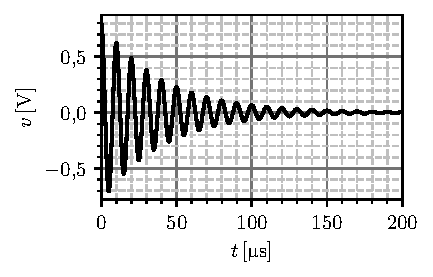
\includegraphics[scale=1]{fig/H_step.pdf}
        \caption{Одкочни одзив у временском домену}
        \label{fig:\ID:step}
    \end{subfigure}
    \caption{Уз решење.}
\end{figure}

(г) Пошто је у питању резонантни систем са уским пропусним опсегом, одзив на одскочну побуду 
јесу осцилације које се временом смирују до нуле. Учестаност тих осцилација је $\upomega_0$, док временска
константа тог процеса одговара реалном делу полова система $\uptau = -1/\upsigma$, где су 
$s = \upsigma \pm \jj\upomega$. Решавањем квадратне једначине \eqref{eq:\ID:std_form} по $s$ добија се 
реални део од приближно $\upsigma = -\dfrac{\upomega_0}{2Q} \approx -35,7\unit{\dfrac{krad}{s}}$ односно
$\uptau \approx 28\unit{\upmu s}$. Узимајући у обзир фреквенцију и временску константу осцилација, добија се 
график приказан на слици \ref{fig:\ID:step}.
